% Genome Biology — Additional file 1
% Supplementary Tables and Figures
% Compile: pdflatex supplementary && pdflatex supplementary
\documentclass[onecolumn]{article}

\usepackage[utf8]{inputenc}
\usepackage[T1]{fontenc}
\usepackage{amsmath,amssymb,amsfonts}
\usepackage{graphicx}
\usepackage{booktabs}
\usepackage[margin=1in]{geometry}
\usepackage{caption}
\usepackage{subcaption}
\usepackage{hyperref}
\usepackage{siunitx}
\usepackage{float}
\usepackage{xcolor}
\usepackage{multirow}
\usepackage{xr}
% Import labels from main.aux so \ref{tab:full18}, \ref{sec:hyperparam} resolve
% in supplementary captions. Requires main.aux to exist (compile main.tex first).
\externaldocument{main}

% Prevent overfull hboxes
\tolerance=1000
\emergencystretch=1em

% Prefix table/figure counters with S
\renewcommand{\thetable}{S\arabic{table}}
\renewcommand{\thefigure}{S\arabic{figure}}

\title{\textbf{Additional file 1 --- Supplementary tables and figures for}\\[6pt]
\textit{Sparse autoencoders reveal organized biological knowledge but minimal regulatory logic in single-cell foundation models: a comparative atlas of Geneformer and scGPT}}

\author{Ihor Kendiukhov}

\date{}

\begin{document}

\maketitle

This file contains supplementary tables and figures for the main manuscript.

\tableofcontents

\clearpage


%% ============================================================
%% SUPPLEMENTARY TABLES
%% ============================================================
\section{Supplementary Tables}

%% --- Table S1: Per-ontology enrichment counts ---
\begin{table}[H]
\centering
\caption{\textbf{Per-ontology enrichment counts across all 18 Geneformer layers.} Each entry is the number of significant enrichments (FDR $< 0.05$) for features at that layer. GO~BP = Gene Ontology Biological Process. TRRUST columns show enrichment for TF target sets (TF) and individual TF$\to$target edges (Edges).}
\label{tab:perontology}
\smallskip
\begin{tabular}{rrrrrrc}
\toprule
Layer & GO BP & KEGG & Reactome & STRING & TRRUST TF & TRRUST Edges \\
\midrule
0  & 10,153 & 2,650 & 11,001 & 302 & 155 & 42 \\
1  & 10,022 & 2,433 & 10,512 & 258 & 164 & 48 \\
2  & 9,948  & 2,495 & 10,790 & 283 & 150 & 32 \\
3  & 9,726  & 2,514 & 9,525  & 273 & 157 & 37 \\
4  & 8,537  & 2,045 & 9,195  & 248 & 133 & 30 \\
5  & 7,695  & 1,845 & 8,189  & 216 & 136 & 24 \\
6  & 7,180  & 1,555 & 7,871  & 182 & 110 & 28 \\
7  & 6,628  & 1,637 & 7,080  & 181 & 125 & 30 \\
8  & 6,850  & 1,570 & 7,169  & 199 & 90  & 27 \\
9  & 7,299  & 1,643 & 7,880  & 207 & 103 & 29 \\
10 & 8,461  & 1,751 & 9,247  & 214 & 128 & 30 \\
11 & 8,785  & 2,089 & 8,957  & 227 & 112 & 31 \\
12 & 8,217  & 1,915 & 8,856  & 210 & 117 & 35 \\
13 & 7,158  & 1,686 & 8,393  & 202 & 101 & 28 \\
14 & 7,615  & 1,595 & 8,412  & 221 & 97  & 27 \\
15 & 6,790  & 1,520 & 7,135  & 150 & 126 & 34 \\
16 & 7,040  & 1,781 & 7,172  & 158 & 87  & 25 \\
17 & 7,002  & 1,762 & 6,869  & 193 & 131 & 25 \\
\midrule
\textbf{Total} & \textbf{145,106} & \textbf{34,486} & \textbf{154,253} & \textbf{3,924} & \textbf{2,222} & \textbf{562} \\
\bottomrule
\end{tabular}
\end{table}


%% --- Table S2: Cross-layer persistence ---
\begin{table}[H]
\centering
\caption{\textbf{Cross-layer feature persistence from layer~0.} Matches = features at L0 with cosine similarity $> 0.7$ to any feature at the target layer. The model undergoes radical representational transformation: by layer~6, essentially all features are novel with no L0 ancestry.}
\label{tab:persistence}
\smallskip
\begin{tabular}{lcc}
\toprule
L0 $\to$ Target & Matches (cos $> 0.7$) & Rate \\
\midrule
L0 $\to$ L1  & 114 & 2.5\% \\
L0 $\to$ L2  & 93 & 2.0\% \\
L0 $\to$ L4  & 67 & 1.5\% \\
L0 $\to$ L6  & 25 & 0.5\% \\
L0 $\to$ L8  & 10 & 0.2\% \\
L0 $\to$ L10 & 1 & $\sim$0\% \\
L0 $\to$ L12+ & 0 & 0\% \\
\bottomrule
\end{tabular}
\end{table}


%% --- Table S3: Co-activation module statistics ---
\begin{table}[H]
\centering
\caption{\textbf{Co-activation module statistics across all 18 layers.} PMI-based graphs with Leiden clustering (resolution = 1.0). Modules = number of distinct communities. Coverage = fraction of alive features in at least one module.}
\label{tab:modules_full}
\smallskip
\begin{tabular}{rccrc}
\toprule
Layer & Modules & Feats in Modules & PMI Edges & Coverage \\
\midrule
0  & 6  & 4,577 & 446,324 & 99.3\% \\
1  & 8  & 4,562 & 440,681 & 99.0\% \\
2  & 7  & 4,536 & 404,403 & 98.6\% \\
3  & 8  & 4,518 & 393,574 & 98.3\% \\
4  & 9  & 4,502 & 393,194 & 98.2\% \\
5  & 12 & 4,472 & 390,845 & 97.7\% \\
6  & 7  & 4,458 & 383,033 & 97.3\% \\
7  & 8  & 4,439 & 371,832 & 96.7\% \\
8  & 7  & 4,478 & 369,280 & 97.6\% \\
9  & 7  & 4,535 & 380,304 & 98.7\% \\
10 & 9  & 4,571 & 388,498 & 99.3\% \\
11 & 8  & 4,565 & 388,103 & 99.3\% \\
12 & 7  & 4,567 & 388,977 & 99.5\% \\
13 & 7  & 4,561 & 383,779 & 99.5\% \\
14 & 8  & 4,543 & 379,595 & 99.5\% \\
15 & 8  & 4,461 & 340,269 & 98.2\% \\
16 & 8  & 4,358 & 327,895 & 96.0\% \\
17 & 7  & 4,474 & 343,059 & 97.7\% \\
\midrule
\textbf{Total} & \textbf{141} & & & \\
\bottomrule
\end{tabular}
\end{table}


%% --- Table S4: Top 10 causal features ---
\begin{table}[H]
\centering
\caption{\textbf{Top 10 causally specific SAE features at layer~11.} $\Delta$Target and $\Delta$Other = mean logit change at target and off-target gene positions, respectively, upon zeroing the feature. Specificity ratios were computed from unrounded values; displayed $\Delta$ values are rounded to three decimal places.}
\label{tab:causal_top10}
\smallskip
\begin{tabular}{clccc}
\toprule
Feature & Annotation & Specificity & $\Delta$Target & $\Delta$Other \\
\midrule
F2035 & Cell Differentiation (neg.\ reg.) & 114.5$\times$ & $-$0.208 & $+$0.002 \\
F3692 & ERAD Pathway & 108.1$\times$ & $-$0.129 & $-$0.001 \\
F3933 & Intracellular Signaling (neg.\ reg.) & 55.7$\times$ & $-$0.196 & $-$0.004 \\
F157  & Golgi Vesicle Transport & 25.4$\times$ & $-$0.056 & $-$0.002 \\
F3532 & Protein Metabolic Process (pos.\ reg.) & 11.2$\times$ & $-$0.127 & $-$0.011 \\
F4516 & Mitotic Spindle Microtubules & 10.6$\times$ & $+$0.672 & $+$0.063 \\
F1337 & Cell Cycle Phase Transition & 9.4$\times$ & $-$0.058 & $-$0.006 \\
F1023 & Mitotic Spindle Microtubules & 7.6$\times$ & $-$2.799 & $-$0.367 \\
F2936 & Mitochondrion Organization & 7.1$\times$ & $-$0.366 & $-$0.051 \\
F3962 & Endocytosis & 6.9$\times$ & $-$0.099 & $-$0.014 \\
\bottomrule
\end{tabular}
\end{table}


%% --- Table S5: Geneformer information highways ---
\begin{table}[H]
\centering
\caption{\textbf{Geneformer cross-layer information highways.} PMI between SAE feature activations at source and target layers (500K positions each). A highway = source feature with $\geq$1 target-layer feature at PMI $> 3$. \textbf{Note:} the numbers here use the main-atlas 500K-position protocol; Table~\ref{tab:highways_null} reports the same three pairs recomputed on a 100K-position subsample with a permutation-null control. The two sets of numbers differ by less than one percentage point (e.g.\ L0$\to$L5: 98.4\% here vs.\ 98.96\% in Table~\ref{tab:highways_null}) because of the different subsample sizes, and the null correction does not change the 100K numbers.}
\label{tab:highways}
\smallskip
\begin{tabular}{lccccc}
\toprule
Layer Pair & Feats w/ Deps & Mean Max PMI & Median Max PMI & Max PMI & Highways \\
\midrule
L0 $\to$ L5   & 4,604 & 6.61 & 6.72 & 11.10 & 4,530 (98.4\%) \\
L5 $\to$ L11  & 4,518 & 6.63 & 6.71 & 10.87 & 4,401 (97.4\%) \\
L11 $\to$ L17 & 4,555 & 6.79 & 6.86 & 10.66 & 4,544 (99.8\%) \\
\bottomrule
\end{tabular}
\end{table}


%% --- Table S6: scGPT information highways ---
\begin{table}[H]
\centering
\caption{\textbf{scGPT cross-layer information highways.} Same methodology as Table~\ref{tab:highways}. Note the progressive drop in downstream connectivity.}
\label{tab:scgpt_highways}
\smallskip
\begin{tabular}{lrccc}
\toprule
Layer Pair & PMI Edges & Upstream & Downstream & Max PMI \\
\midrule
L0 $\to$ L4  & 75,305 & 1,935/2,027 (95.5\%) & 1,960/2,048 (95.7\%) & 9.15 \\
L4 $\to$ L8  & 61,263 & 1,955/2,048 (95.5\%) & 1,723/2,048 (84.1\%) & 9.26 \\
L8 $\to$ L11 & 45,258 & 1,773/2,048 (86.6\%) & 1,289/2,048 (62.9\%) & 10.78 \\
\bottomrule
\end{tabular}
\end{table}


%% --- Table S7: Biological cascades ---
\begin{table}[H]
\centering
\caption{\textbf{Top cross-layer biological cascades.} Strongest annotated PMI connections between layer pairs. ``Unlabeled'' = the target feature lacks direct ontology annotation.}
\label{tab:cascades}
\smallskip
\small
\begin{tabular}{lp{2.6cm}p{2.6cm}p{3.2cm}r}
\toprule
Pair & Source Feature & Target Feature & Biological Logic & PMI \\
\midrule
L0$\to$L5  & Protein Processing in ER & \textit{unlabeled} & ER stress cascade & 11.10 \\
L0$\to$L5  & mTORC1 Regulation & Autophagy & mTORC1$\to$autophagy & 9.55 \\
L0$\to$L5  & Wnt Signaling & \textit{unlabeled} & Wnt pathway processing & 9.48 \\
\midrule
L5$\to$L11 & Protein Polyubiq. & \textit{unlabeled} & Protein quality control & 10.87 \\
L5$\to$L11 & Translation & \textit{unlabeled} & Translational regulation & 10.35 \\
L5$\to$L11 & RNA Splicing (neg.\ reg.) & \textit{unlabeled} & Post-transcriptional & 10.21 \\
\midrule
L11$\to$L17 & Protein Modification & Angiogenesis (pos.\ reg.) & PTM$\to$phenotype & 10.62 \\
L11$\to$L17 & COPII Vesicle Budding & Thermogenesis & Secretory$\to$metabolic & 10.29 \\
L11$\to$L17 & Actomyosin Org. & Cell Locomotion (neg.\ reg.) & Structure$\to$motility & 10.14 \\
\bottomrule
\end{tabular}
\end{table}


%% --- Table S8: Per-TF comparison ---
\begin{table}[H]
\centering
\caption{\textbf{Per-TF head-to-head comparison at layer~11.} Only TFs with changed specificity are shown; 40 additional TFs had no specific features in either condition.}
\label{tab:per_tf}
\smallskip
\begin{tabular}{lccc}
\toprule
TF & K562-SAE Specific & MT-SAE Specific & Change \\
\midrule
ATF5  & 0 & 1 & gained \\
BRCA1 & 0 & 1 & gained \\
GATA1 & 0 & 1 & gained \\
RBMX  & 0 & 1 & gained \\
NFRKB & 0 & 1 & gained \\
\midrule
MAX   & 1 & 0 & lost \\
PHB2  & 1 & 0 & lost \\
SRF   & 1 & 0 & lost \\
\bottomrule
\end{tabular}
\end{table}


%% --- Table S9: TF diagnostics ---
\begin{table}[H]
\centering
\caption{\textbf{TF feature diagnostics.} Features with known TFs in top-20 genes and TF-dominant features ($\geq$3 TFs in top genes). Denominators = features with non-empty top-20 gene lists (may differ from alive counts because some features that are ``dead'' on the 100K held-out sample still produce gene lists from the full training data). K562-only SAE has more TF-associated features than the multi-tissue SAE.}
\label{tab:tf_diagnostics}
\smallskip
\begin{tabular}{lcc}
\toprule
SAE & Features with TFs in top genes & TF-dominant ($\geq$3 TFs) \\
\midrule
K562-only L11     & 2,967/4,598 (64.5\%) & 424 \\
Multi-tissue L0   & 2,796/4,608 (60.7\%) & 452 \\
Multi-tissue L5   & 2,777/4,568 (60.8\%) & 337 \\
Multi-tissue L11  & 2,782/4,601 (60.5\%) & 343 \\
Multi-tissue L17  & 2,680/4,603 (58.2\%) & 346 \\
\bottomrule
\end{tabular}
\end{table}


%% --- Table S10: Novel/unannotated features ---
\begin{table}[H]
\centering
\caption{\textbf{Unannotated feature analysis (original preprint).} Co-activate = unannotated feature belongs to a co-activation module containing annotated features. Isolated = no module membership. A small number of features (3 at L11, 17 at L17) belong to modules containing only unannotated features and are excluded from both columns. Clusters = standalone gene-set clusters among unannotated features. As discussed in \S2.11 of the main text, the co-activate/isolated column is now regarded as weak evidence (modules cover 96--99.5\% of all features so co-membership is nearly unavoidable) and is retained here only for completeness. The more informative tests appear in Table~\ref{tab:unannotated_new}.}
\label{tab:novel}
\smallskip
\begin{tabular}{rrrcrr}
\toprule
Layer & Annotated & Unannotated & Clusters & Co-activate w/ Annotated & Isolated \\
\midrule
0  & 2,702 & 1,906 & 15 (48 feats) & 1,876 (98.4\%) & 30 (1.6\%) \\
5  & 2,383 & 2,193 & 19 (69 feats) & 2,090 (95.3\%) & 103 (4.7\%) \\
11 & 2,583 & 2,015 & 11 (47 feats) & 1,984 (98.5\%) & 28 (1.4\%) \\
17 & 2,154 & 2,426 & 12 (58 feats) & 2,334 (96.2\%) & 75 (3.1\%) \\
\bottomrule
\end{tabular}
\end{table}


%% --- Table S-SVD: SVD threshold sensitivity ---
\begin{table}[H]
\centering
\caption{\textbf{Sensitivity of the SAE-vs-SVD comparison to the cosine threshold (Geneformer, all 18 layers).} For each layer and each cosine threshold $\tau \in \{0.3, 0.5, 0.7, 0.9\}$: percentage of alive SAE features whose decoder column has maximum absolute cosine above $\tau$ with any of the top-50 SVD axes (columns ``aligned\%''), and percentage of ontology enrichments found exclusively in the non-aligned (``novel'') set (columns ``\%enrich novel''). The value $\tau{=}0.5$ reproduces the per-layer SVD-aligned counts in Table~\ref{tab:full18} (the original preprint quoted $\tau{=}0.7$ in the text but the pipeline actually used $\tau{=}0.5$; we have corrected the main text). Across the full range, $>98\%$ of ontology enrichments live exclusively in the novel set, so the headline conclusion is robust.}
\label{tab:svd_sweep}
\smallskip
\small
\begin{tabular}{r|rrrr|rrrr}
\toprule
& \multicolumn{4}{c|}{Aligned \%} & \multicolumn{4}{c}{\% enrich in novel} \\
Layer & $\tau{=}0.3$ & $\tau{=}0.5$ & $\tau{=}0.7$ & $\tau{=}0.9$ & $\tau{=}0.3$ & $\tau{=}0.5$ & $\tau{=}0.7$ & $\tau{=}0.9$ \\
\midrule
0  & 4.19 & 0.89 & 0.02 & 0.00 & 98.88 & 99.98 & 100.00 & 100.00 \\
1  & 3.45 & 0.59 & 0.07 & 0.00 & 99.54 & 99.98 & 100.00 & 100.00 \\
2  & 3.73 & 0.63 & 0.04 & 0.00 & 99.49 & 99.93 & 100.00 & 100.00 \\
3  & 3.26 & 0.26 & 0.00 & 0.00 & 99.27 & 100.00 & 100.00 & 100.00 \\
4  & 2.69 & 0.28 & 0.00 & 0.00 & 99.48 & 99.97 & 100.00 & 100.00 \\
5  & 2.63 & 0.17 & 0.00 & 0.00 & 98.92 & 100.00 & 100.00 & 100.00 \\
6  & 2.39 & 0.11 & 0.00 & 0.00 & 98.62 & 99.99 & 100.00 & 100.00 \\
7  & 2.08 & 0.13 & 0.00 & 0.00 & 98.30 & 99.99 & 100.00 & 100.00 \\
8  & 1.48 & 0.07 & 0.00 & 0.00 & 99.40 & 99.98 & 100.00 & 100.00 \\
9  & 1.09 & 0.09 & 0.00 & 0.00 & 99.36 & 99.99 & 100.00 & 100.00 \\
10 & 1.09 & 0.15 & 0.00 & 0.00 & 99.63 & 100.00 & 100.00 & 100.00 \\
11 & 0.74 & 0.09 & 0.00 & 0.00 & 99.28 & 100.00 & 100.00 & 100.00 \\
12 & 0.65 & 0.07 & 0.00 & 0.00 & 99.26 & 100.00 & 100.00 & 100.00 \\
13 & 0.95 & 0.07 & 0.00 & 0.00 & 98.75 & 100.00 & 100.00 & 100.00 \\
14 & 0.93 & 0.04 & 0.00 & 0.00 & 97.90 & 99.55 & 100.00 & 100.00 \\
15 & 1.09 & 0.11 & 0.00 & 0.00 & 98.28 & 99.03 & 100.00 & 100.00 \\
16 & 1.00 & 0.11 & 0.02 & 0.00 & 98.73 & 99.02 & 99.47 & 100.00 \\
17 & 1.63 & 0.26 & 0.02 & 0.00 & 98.68 & 99.99 & 100.00 & 100.00 \\
\bottomrule
\end{tabular}
\end{table}


%% --- Table S-PMI: graph dimensions and memory ---
\begin{table}[H]
\centering
\caption{\textbf{PMI co-activation graph dimensions and peak memory (Geneformer layers 0 and 11).} Recomputed on a deterministic 500{,}000-position subsample (seed 42) of the 4{,}056{,}351 K562 token positions at each layer, with $\texttt{MIN\_COACTIVATION}{=}20$ and $\texttt{PMI\_THRESHOLD}{=}2.0$ to match the main-text co-activation pipeline (main-text numbers use the full 4M positions with $\texttt{MIN\_COACTIVATION}{=}50$). $N_\text{feat}$ = alive features at the layer. Peak RSS measured with \texttt{psutil.Process().memory\_info().rss}. The dense ($N{\times}N$) coactivation matrix accounts for $\approx$85~MB of the budget; the remaining $\sim$700~MB is the subsampled TopK index buffer and PyTorch/Python overhead.}
\label{tab:pmi_memory}
\smallskip
\small
\begin{tabular}{rrrrrrrr}
\toprule
Layer & $N_\text{feat}$ & Subsampled positions & $|E|$ (after thresh.) & Coact matrix (MB) & Peak RSS (MB) & Encode (s) & PMI (s) \\
\midrule
0  & 4{,}608 & 500{,}000 & 435{,}252 & 85 & 811 & 100.1 & 11.0 \\
11 & 4{,}608 & 500{,}000 & 356{,}894 & 85 & 864 &  93.6 & 10.3 \\
\bottomrule
\end{tabular}
\end{table}


%% --- Table S-Leiden: resolution sweep ---
\begin{table}[H]
\centering
\caption{\textbf{Leiden resolution sweep at Geneformer layers 0 and 11.} Module count ($\geq$3 features), mean module size, coverage (fraction of graph nodes in $\geq$3-feature modules), and Adjusted Rand Index vs.\ the baseline $\gamma{=}1.0$ partition for $\gamma \in \{0.5, 0.75, 1.0, 1.5, 2.0\}$. \textbf{Note on comparison with Table~\ref{tab:modules_full}:} this sweep is run on a deterministic 500K-position subsample with $\texttt{MIN\_COACTIVATION}{=}20$ (see caption of Table~\ref{tab:pmi_memory}), whereas the main-text module counts in Table~\ref{tab:modules_full} use the full 4{,}056{,}351 positions with $\texttt{MIN\_COACTIVATION}{=}50$. The different PMI significance thresholds produce slightly different partition sizes; at $\gamma{=}1.0$ the sweep gives 8 modules at L0 and 9 at L11, versus 6 and 8 in Table~\ref{tab:modules_full}. This disagreement is expected given the parameter change and should not be read as instability. The partition is \emph{not} stable in a strong ARI sense (ARI between $\gamma{=}1.0$ and its immediate neighbors is in the 0.17--0.26 range); instead, the co-activation graph exhibits a nested hierarchy in which low $\gamma$ collapses the graph into $\sim$2 very large communities and high $\gamma$ fragments each main community into finer subcommunities. The qualitative biological identities of modules (cell cycle, translation, metabolism, etc.) are preserved across the range; our main-text module counts correspond to the resolution-1.0 cut of this hierarchy.}
\label{tab:leiden_sweep}
\smallskip
\small
\begin{tabular}{rrrrrr}
\toprule
Layer & $\gamma$ & Modules ($\geq$3) & Mean size & Coverage & ARI vs $\gamma{=}1.0$ \\
\midrule
0  & 0.50 &  2 & 2{,}287.5 & 100.0\% & +0.027 \\
0  & 0.75 &  3 & 1{,}525.0 & 100.0\% & +0.259 \\
0  & 1.00 &  8 &    571.9 & 100.0\% & +1.000 \\
0  & 1.50 & 25 &    183.0 & 100.0\% & +0.252 \\
0  & 2.00 & 48 &     95.3 & 100.0\% & +0.117 \\
\midrule
11 & 0.50 &  2 & 2{,}282.0 & 100.0\% & +0.013 \\
11 & 0.75 &  3 & 1{,}521.3 & 100.0\% & +0.180 \\
11 & 1.00 &  9 &    507.1 & 100.0\% & +1.000 \\
11 & 1.50 & 31 &    147.2 & 100.0\% & +0.171 \\
11 & 2.00 & 56 &     81.5 & 100.0\% & +0.085 \\
\bottomrule
\end{tabular}
\end{table}


%% --- Table S-Hyperparam: expansion x k grid ---
\begin{table}[H]
\centering
\caption{\textbf{SAE hyperparameter ablation at Geneformer layer~11.} Grid over expansion ratio $\in \{2\times, 4\times, 8\times\}$ and TopK sparsity $k \in \{16, 32, 64\}$, trained on the same 1M-position K562 subsample used in the main atlas (Methods), evaluated on 100K held-out positions. Columns: expansion, $k$, total features, variance explained on held-out positions, number of dead features (no activation on the 100K hold-out), mean absolute decoder--decoder cosine similarity on a 5{,}000-pair sample (a proxy for quasi-orthogonality), and Leiden module count ($\geq$3 features, $\gamma{=}1.0$) on a 200K-position co-activation graph. The baseline configuration ($4\times$, $k{=}32$) sits at the center of the grid and does not produce an unusual point: variance explained increases monotonically with both expansion and $k$, module count is within 7--12 across the entire grid, and quasi-orthogonality is preserved everywhere ($\langle|\cos|\rangle \lesssim 0.05$). The main-text qualitative conclusions---substantial superposition, organized biological structure, modular co-activation---are preserved across the grid. We report the structural metrics here; full downstream annotation rate and TF specificity per grid cell are beyond this revision's compute budget (see \S\ref{sec:hyperparam}).}
\label{tab:hyperparam}
\smallskip
\small
\begin{tabular}{rrrrrrr}
\toprule
Expansion & $k$ & $N_\text{feat}$ & VarExpl & Dead & $\langle|\cos|\rangle$ & Modules ($\geq$3) \\
\midrule
$2\times$ & 16 & 2{,}304 & 0.706 &  95 & 0.0421 &  9 \\
$2\times$ & 32 & 2{,}304 & 0.752 &  11 & 0.0383 & 10 \\
$2\times$ & 64 & 2{,}304 & 0.795 &   1 & 0.0338 &  8 \\
$4\times$ & 16 & 4{,}608 & 0.790 & 228 & 0.0394 & 12 \\
\textbf{$4\times$} & \textbf{32} & \textbf{4{,}608} & \textbf{0.819} & \textbf{45}  & \textbf{0.0365} & \textbf{7} \\
$4\times$ & 64 & 4{,}608 & 0.846 &   1 & 0.0327 &  7 \\
$8\times$ & 16 & 9{,}216 & 0.846 & 559 & 0.0360 & 12 \\
$8\times$ & 32 & 9{,}216 & 0.866 & 112 & 0.0345 &  8 \\
$8\times$ & 64 & 9{,}216 & 0.884 &   8 & 0.0329 &  6 \\
\bottomrule
\end{tabular}
\\[2pt]
\footnotesize Bold row: main-atlas baseline used in Table~\ref{tab:full18} and throughout the paper.
\end{table}


%% --- Table S-ScGPTpert: scGPT perturbation specificity on Replogle ---
\begin{table}[H]
\centering
\caption{\textbf{scGPT perturbation response mapping on Replogle K562 CRISPRi, layer~7.} 50 perturbation targets (top of the same target list used in the Geneformer Table~6 test), 10 cells per target, 100 non-targeting K562 control cells, per-cell binned expression values re-tokenized from the Replogle source h5ad. Responding features = mean activation effect size vs.\ control $|z| > 0.5$. ``Specific'' definitions match Table~\ref{tab:regulatory_dbs}. Both TRRUST and DoRothEA~A+B+C yield single-digit loose overlap rates, and zero FDR-corrected specific TFs---in the same qualitative regime as the Geneformer L11 numbers in Table~\ref{tab:regulatory_dbs}.}
\label{tab:scgpt_pert}
\smallskip
\small
\begin{tabular}{lrrrrrr}
\toprule
Database & DB TFs & In panel & Loose $n$ & Loose rate & FDR$<$0.05 $n$ & FDR rate \\
\midrule
TRRUST           & 795 & 28 & 2 & 7.14\% & 0 & 0.00\% \\
DoRothEA (A+B+C) & 429 & 12 & 2 & 16.67\% & 0 & 0.00\% \\
\bottomrule
\end{tabular}
\end{table}


%% --- Table S-Regulatory: multi-database perturbation ---
\begin{table}[H]
\centering
\caption{\textbf{Perturbation specificity across regulatory databases.} Same experimental protocol as Table~6 of the main text (Geneformer L11 SAE, Replogle CRISPRi, 100 perturbation targets) but tested against three regulatory priors: TRRUST (Han et al., 2018; literature-mined), DoRothEA A+B+C (Garcia-Alonso et al., 2019; high-confidence subset), and DoRothEA all (all confidence levels). Columns: database, total TFs in the database, TFs present in the Replogle panel with $\geq$5 known targets, number of TFs with at least one responding feature whose top-20 gene list overlaps a known target (``loose''), loose rate, number with a significant hypergeometric enrichment of their known targets in the union top-20 gene list across responding features (BH-corrected FDR$<$0.05 across the TF panel, universe $=$ 20,000 human protein-coding genes), and FDR rate. The ``loose'' column climbs with database size because larger target sets make coincidental overlaps more likely; the FDR-corrected column, which controls for target-set size via the hypergeometric test, stays in the single-digit range across all three databases. Note: the loose TRRUST rate of 3.57\% here (1/28) applies the same $\geq$5-known-targets cutoff used for DoRothEA; the 6.2\% headline rate in Table~6 of the main text uses the main-text pipeline's feature-level definition of ``specific response'' and a 48-TF panel with no $\geq$5 cutoff.}
\label{tab:regulatory_dbs}
\smallskip
\small
\begin{tabular}{lrrrrrr}
\toprule
Database & DB TFs & In panel & Loose $n$ & Loose rate & FDR$<$0.05 $n$ & FDR rate \\
\midrule
TRRUST           & 795 & 28 & 1 & 3.57\% & 0 & 0.00\% \\
DoRothEA (A+B+C) & 429 & 12 & 4 & 33.33\% & 1 & 8.33\% \\
DoRothEA (all)   & 643 & 18 & 7 & 38.89\% & 1 & 5.56\% \\
\bottomrule
\end{tabular}
\end{table}


%% --- Table S-CausalTrue: scGPT true-value causal patching ---
\begin{table}[H]
\centering
\caption{\textbf{scGPT causal patching at layer~7: proxy (uniform 1.0) vs.\ true binned expression values.} Lean head-to-head on a 20-cell $\times$ 10-feature subset drawn from the Tabula Sapiens extraction panel, with features re-tokenized from the source h5ad files (\texttt{tabula\_sapiens\_\{immune,kidney,lung\}.h5ad}) to recover the per-cell binned values. Specificity is measured as a simplified layer-7 SAE reconstruction delta after single-feature ablation (not final-layer logit change), so the absolute numbers are not directly comparable to the 0.98$\times$ figure in \S2.7 of the main text; the comparison between the two modes is, however, controlled. Results are essentially identical between the two input regimes, indicating that the preprint's low scGPT causal specificity is \emph{not} an artifact of the uniform-value proxy.}
\label{tab:causal_true}
\smallskip
\small
\begin{tabular}{lrrrr}
\toprule
Mode & Median specificity & Mean specificity & Max specificity & $\#$ features $>2\times$ \\
\midrule
Proxy (uniform 1.0)      & 0.000 & 1.657 & 7.062 & 3 \\
True (per-cell bins) & 0.000 & 1.631 & 6.730 & 3 \\
\bottomrule
\end{tabular}
\end{table}


%% --- Table S-Highways: null-corrected cross-layer highways ---
\begin{table}[H]
\centering
\caption{\textbf{Null-corrected cross-layer highway fractions for the three long-range Geneformer pairs.} 100K gene positions subsampled from the K562 activation cache, encoded through the per-layer SAEs, cross-layer PMI computed as in Methods. Columns: observed 99th percentile of cross-layer PMI, permutation-null 99th percentile ($\tau_{\text{null}}^{p99}$, max across 20 column-shuffle rounds), effective threshold $\tau = \max(3.0, \tau_{\text{null}}^{p99})$, and highway fraction. The permutation null's 99th-percentile PMI is \emph{below} 3.0 in every pair tested, so the fixed threshold $\tau{=}3.0$ is already conservative and the null correction leaves the highway fraction unchanged. This argues that the $\sim$97--99\% highway rate is not an artifact of the $k{=}32$ TopK sparsity.}
\label{tab:highways_null}
\smallskip
\small
\begin{tabular}{rrrrrrr}
\toprule
Src & Tgt & Obs $p99$ PMI & Null $p99$ PMI & $\tau_\text{eff}$ & Fixed-$\tau$ highway\% & Null-corr highway\% \\
\midrule
L0  & L5  & 4.76 & 2.46 & 3.00 & 98.96\% & 98.96\% \\
L5  & L11 & 4.93 & 2.76 & 3.00 & 96.66\% & 96.66\% \\
L11 & L17 & 4.77 & 2.85 & 3.00 & 99.02\% & 99.02\% \\
\bottomrule
\end{tabular}
\end{table}

%% --- Table S-Highways consecutive: L_i -> L_{i+1} sweep (no permutation) ---
\begin{table}[H]
\centering
\caption{\textbf{Consecutive-layer highway fractions L$_i$$\to$L$_{i+1}$ (Geneformer, fixed-$\tau$).} Same protocol as Table~\ref{tab:highways_null} (100K gene positions per layer, fixed $\tau{=}3.0$). Because the permutation null's 99th percentile PMI is below 3.0 for every long-range pair tested in Table~\ref{tab:highways_null}, we do not re-run the permutation null on every consecutive pair. The curve is near-flat in the 94.7--99.1\% range with no sharp drop at any single transition, supporting continuous cross-layer information flow rather than concentrated bottlenecks. The slight dip at the final layer pair (L16$\to$L17) is consistent with the terminal-layer specialization reported in \S\ref{sec:ushape}.}
\label{tab:highways_consecutive}
\smallskip
\small
\begin{tabular}{rr}
\toprule
L$_i$$\to$L$_{i+1}$ & Highway\% \\
\midrule
L0  $\to$ L1  & 98.68\% \\
L1  $\to$ L2  & 98.74\% \\
L2  $\to$ L3  & 98.48\% \\
L3  $\to$ L4  & 98.35\% \\
L4  $\to$ L5  & 97.70\% \\
L5  $\to$ L6  & 97.09\% \\
L6  $\to$ L7  & 97.55\% \\
L7  $\to$ L8  & 96.96\% \\
L8  $\to$ L9  & 97.37\% \\
L9  $\to$ L10 & 98.24\% \\
L10 $\to$ L11 & 99.13\% \\
L11 $\to$ L12 & 99.05\% \\
L12 $\to$ L13 & 99.05\% \\
L13 $\to$ L14 & 98.87\% \\
L14 $\to$ L15 & 98.48\% \\
L15 $\to$ L16 & 96.72\% \\
L16 $\to$ L17 & 94.70\% \\
\bottomrule
\end{tabular}
\end{table}


%% --- Table S-Unannotated: new non-tautological tests ---
\begin{table}[H]
\centering
\caption{\textbf{Cell-type and perturbation-response tests for unannotated features (Geneformer layers 0, 5, 11, 17).} Columns: \#unann~= number of features with zero ontology enrichments; CT\%~unann~= fraction of those that are enriched for $\geq$1 of the 56 Tabula Sapiens cell types (Fisher's exact, BH FDR$<$0.05); CT\%~ann = same for the annotated population; CT\%~null = expected fraction for a matched random subset of size \#unann drawn from all alive features; Pert\%~unann~= fraction of unannotated features that appear in the top-20 responding list for $\geq$1 of the 100 Replogle CRISPRi targets with $|$effect$| > 0.5$; Pert\%~ann and Pert\%~null defined analogously. Cell-type rates are uniformly high ($\approx 90$--95\%) for both populations, reflecting that nearly every SAE feature at these layers is cell-type-selective in Tabula Sapiens; this test does not separate the two populations cleanly. The perturbation test does separate them: at layer 11 unannotated features are $\sim$15$\times$ more likely than annotated features to appear in a top-20 responding list, providing non-tautological evidence that a subset of unannotated features carry real perturbation-response signal.}
\label{tab:unannotated_new}
\smallskip
\small
\begin{tabular}{rrrrrrrr}
\toprule
Layer & \#unann & CT\% unann & CT\% ann & CT\% null & Pert\% unann & Pert\% ann & Pert\% null \\
\midrule
0  & 1{,}906 & 94.96\% & 94.52\% & 94.70\% & 0.42\% & 0.22\% & 0.30\% \\
5  & 2{,}225 & 91.73\% & 95.80\% & 93.85\% & 2.20\% & 1.72\% & 1.93\% \\
11 & 2{,}025 & 92.94\% & 95.74\% & 94.53\% & 2.32\% & 0.15\% & 1.11\% \\
17 & 2{,}454 & 89.41\% & 94.89\% & 91.96\% & 3.63\% & 3.81\% & 3.70\% \\
\bottomrule
\end{tabular}
\end{table}


%% --- Table S-Matched: matched-input cross-model comparison ---
\begin{table}[H]
\centering
\caption{\textbf{Matched-input Geneformer variance explained at Tabula Sapiens layers 0, 5, 11.} K562-trained Geneformer SAEs applied to the same 3{,}000 Tabula Sapiens cells used for the scGPT atlas (L0, L5, L11 activations already extracted in the phase-3 pipeline). 200K position subsample per layer, variance explained computed on held-out batches without retraining. When Geneformer SAEs see out-of-distribution data (Tabula Sapiens, not K562), variance explained drops by 18--23 percentage points, implying that the 9-percentage-point Geneformer-vs-scGPT variance-explained gap in Table~\ref{tab:model_comparison} of the main text is a lower bound on the architectural gap in Tabula-Sapiens-like distributions: under matched input, the gap widens to $\sim$27 pp (e.g.\ 0.636 Geneformer vs.\ scGPT's 0.886 mean VarExpl at comparable depth). Alive feature counts are essentially unchanged between the two input distributions, meaning this is not a case of SAEs collapsing to a subset of dead units.}
\label{tab:matched}
\smallskip
\small
\begin{tabular}{rrrrrr}
\toprule
Layer & K562 VarExpl & K562 alive & TS-matched VarExpl & TS-matched alive & $\Delta$VarExpl \\
\midrule
0  & 0.846 & 4{,}606 & 0.618 & 4{,}608 & $-$0.228 \\
5  & 0.854 & 4{,}537 & 0.638 & 4{,}539 & $-$0.216 \\
11 & 0.820 & 4{,}577 & 0.636 & 4{,}575 & $-$0.184 \\
\bottomrule
\end{tabular}
\end{table}


%% --- Table S-Batch: donor/assay confound analysis ---
\begin{table}[H]
\centering
\caption{\textbf{scGPT feature mutual-information with tissue vs.\ cell type.} 150K-position subsample at each of scGPT layers \{0, 4, 7, 11\}. ``Tissue-dominant'' = feature whose per-feature MI with tissue (3-way: immune/kidney/lung) exceeds its MI with cell type (56-way). Tissue here is a proxy for sample-level batch because the cached scGPT extraction metadata records only \{tissue, cell\_type\}, not donor ID or sequencing assay. Across all four layers, mean MI with cell type is $\sim$2.5$\times$ larger than mean MI with tissue, and essentially zero features are tissue-dominant. A full donor-level analysis would require joining the Tabula Sapiens source h5ad on cell\_idx; we flag this as a follow-up.}
\label{tab:batch}
\smallskip
\small
\begin{tabular}{rrrrrr}
\toprule
Layer & Alive feats & Mean MI(tissue) & Mean MI(cell\_type) & Tissue-dominant & Frac tissue-dominant \\
\midrule
0  & 1{,}990 & 0.0003 & 0.0008 & 0 & 0.00\% \\
4  & 2{,}038 & 0.0005 & 0.0015 & 0 & 0.00\% \\
7  & 1{,}999 & 0.0009 & 0.0023 & 0 & 0.00\% \\
11 & 1{,}766 & 0.0016 & 0.0040 & 1 & 0.06\% \\
\bottomrule
\end{tabular}
\end{table}


\clearpage


%% ============================================================
%% SUPPLEMENTARY FIGURES
%% ============================================================
\section{Supplementary Figures}


%% --- Figure S1 (was S3): scGPT highways ---
\begin{figure}[H]
\centering
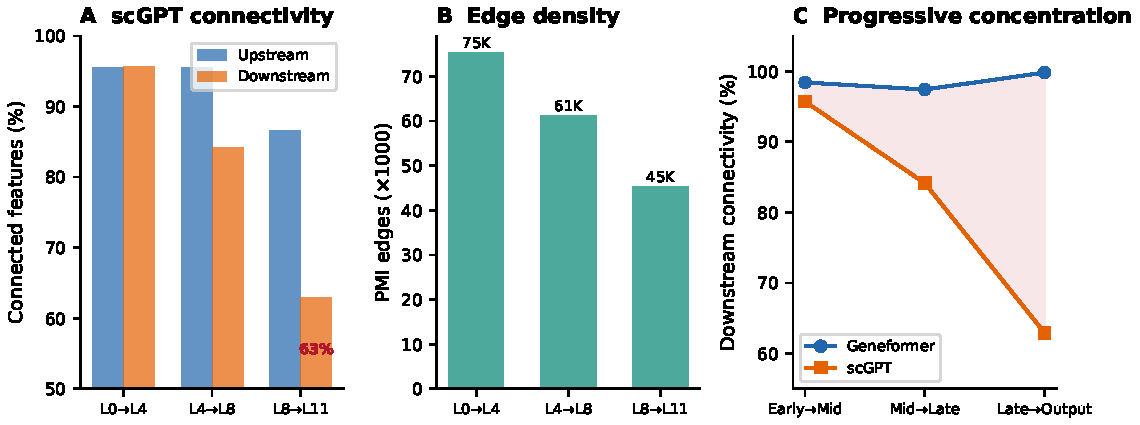
\includegraphics[width=\textwidth]{figures/gb_figS3_scgpt_highways.pdf}
\caption{\textbf{scGPT cross-layer connectivity reveals progressive information concentration.} \textbf{(A)}~Upstream connectivity remains high (86--96\%) but downstream connectivity drops sharply from 96\% to 63\% across layer pairs, indicating progressive bottlenecking. \textbf{(B)}~PMI edge density decreases from 75K to 45K edges across the three layer pairs. \textbf{(C)}~Comparison with Geneformer: Geneformer maintains near-complete downstream connectivity (97--100\%) while scGPT drops to 63\%, suggesting fundamentally different information flow architectures.}
\label{fig:scgpt_highways}
\end{figure}


%% --- Figure S2 (was S4): UMAP/force-directed overview ---
\begin{figure}[H]
\centering
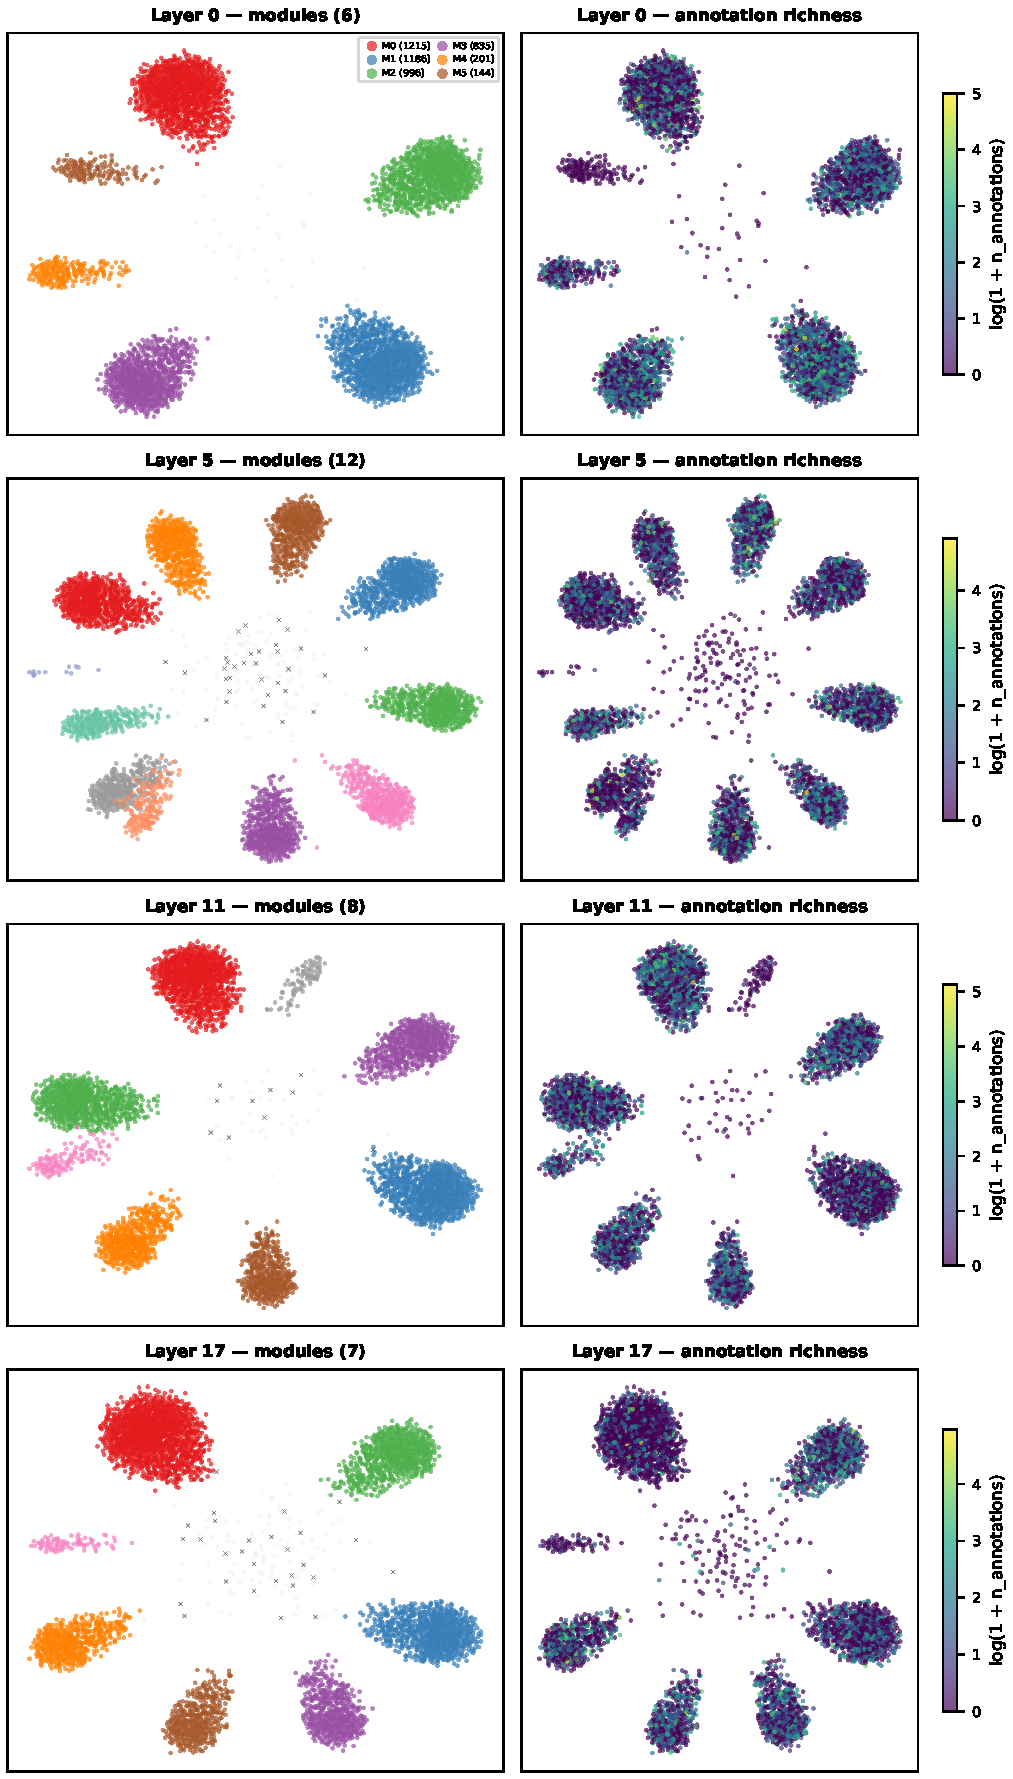
\includegraphics[width=\textwidth,height=0.85\textheight,keepaspectratio]{figures/gb_figS4_umap_overview.pdf}
\caption{\textbf{Co-activation network layout of SAE features across layers.} All panels are \textbf{force-directed (Fruchterman--Reingold) layouts of the intra-module co-activation graph} produced with NetworkX; they are \emph{not} UMAP or t-SNE projections of the feature decoder vectors (which are quasi-orthogonal by construction and therefore produce structureless UMAP point clouds). Left column: nodes colored by Leiden module membership. Each module forms a spatially distinct community. Right column: same layouts colored by annotation richness (log-transformed number of significant enrichment terms). Unassigned features (gray) cluster centrally. Module count varies from 6 (L0) to 12 (L5), reflecting the different co-activation patterns at each layer.}
\label{fig:umap_overview}
\end{figure}


%% --- Figure S3 (was S5): L11 detail ---
\begin{figure}[H]
\centering
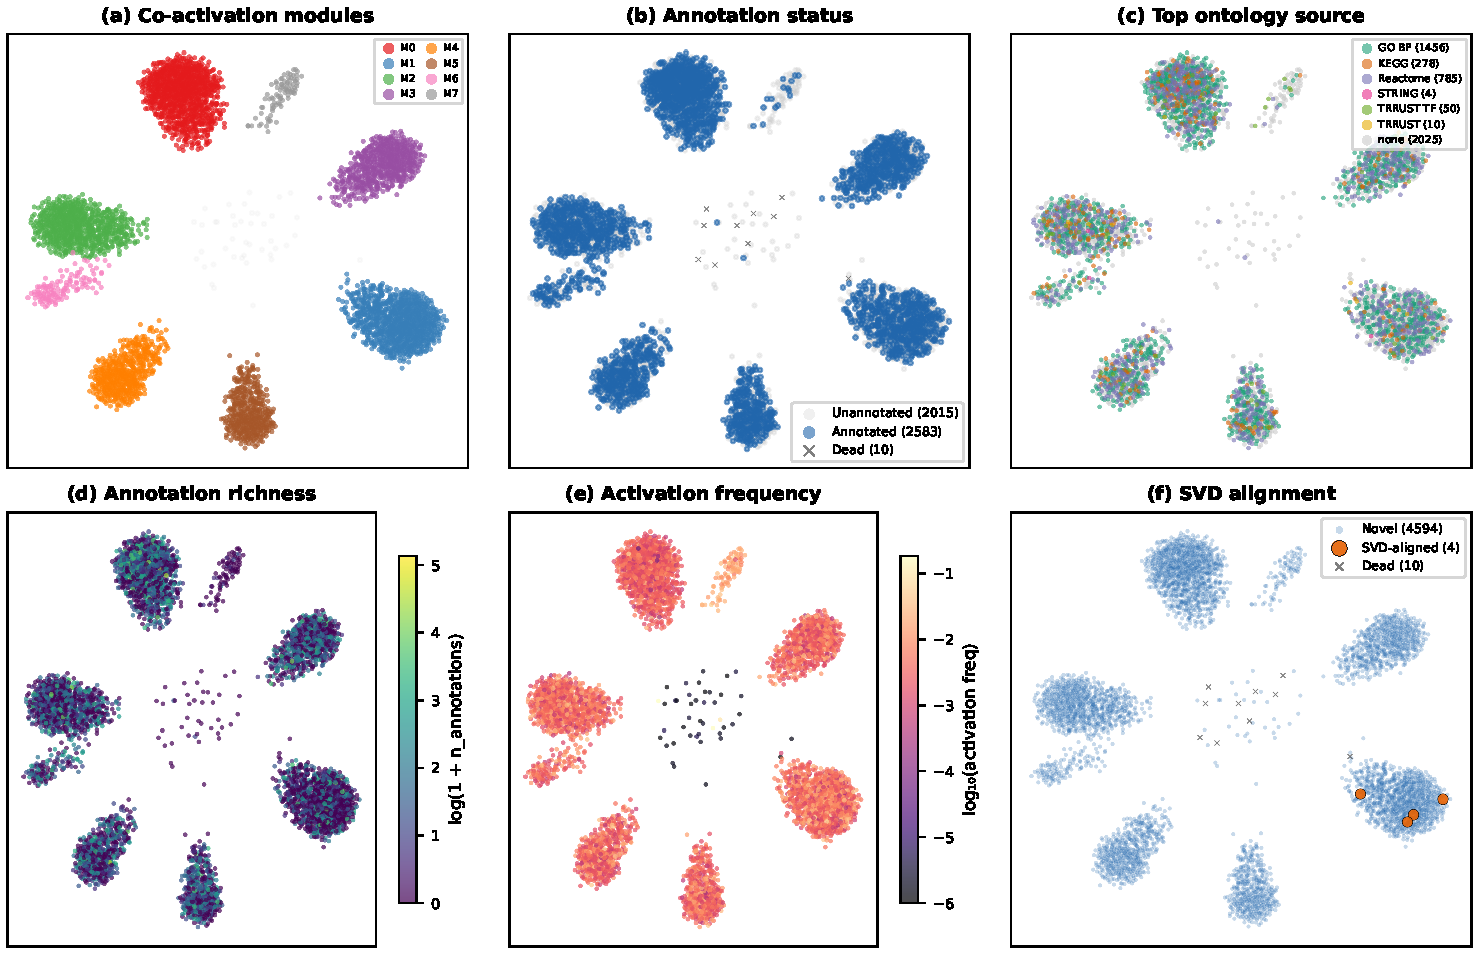
\includegraphics[width=\textwidth]{figures/gb_figS5_l11_detail.pdf}
\caption{\textbf{Six-panel force-directed co-activation layout of layer~11 SAE features.} All six panels share the same \textbf{Fruchterman--Reingold (NetworkX) layout of the intra-module co-activation graph}; the panels differ only in the node-coloring overlay. This is \emph{not} a UMAP, t-SNE, or PCA projection of decoder weight vectors. \textbf{(a)}~Eight Leiden modules form spatially distinct communities. \textbf{(b)}~Annotated features (blue) distribute across all module clusters; unannotated features (gray) concentrate centrally. \textbf{(c)}~Top ontology source reveals module-specific enrichment patterns: certain modules are dominated by GO~BP (green), others by STRING interactions (pink) or Reactome pathways (purple). \textbf{(d)}~Annotation richness gradient across modules. \textbf{(e)}~Activation frequency varies across modules. \textbf{(f)}~SVD-aligned features (orange, $n=4$) are scattered across different modules, while 4,594 novel features (blue) fill the landscape.}
\label{fig:l11_detail}
\end{figure}


%% --- Figure S4 (was S6): Annotation-based projections ---
\begin{figure}[H]
\centering
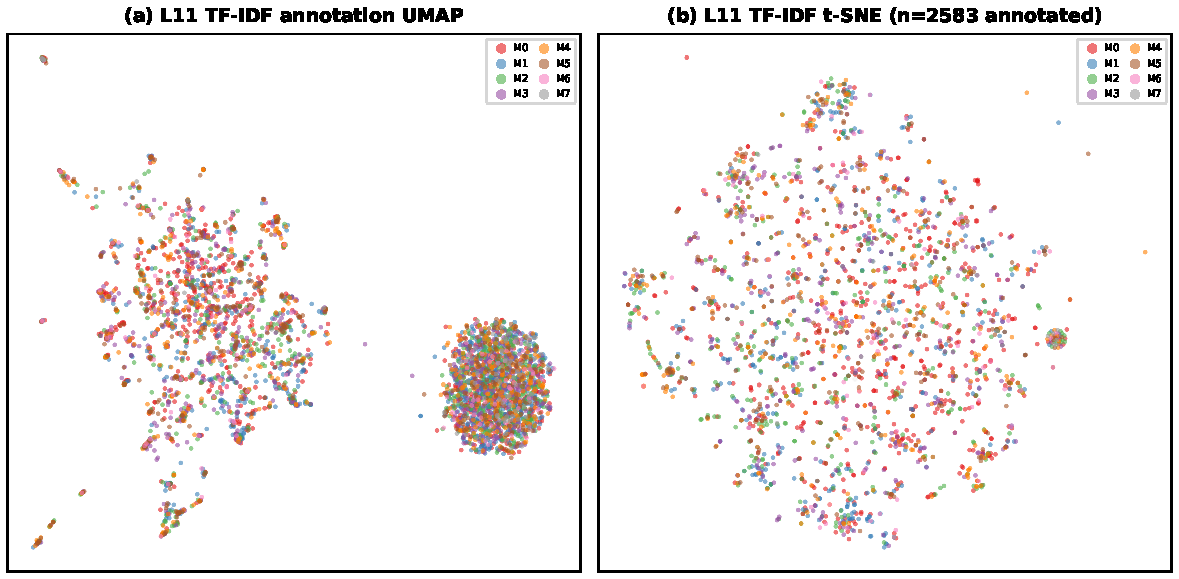
\includegraphics[width=\textwidth]{figures/gb_figS6_annotation_projections.pdf}
\caption{\textbf{Annotation-based projections provide independent validation.} \textbf{(a)}~UMAP of TF-IDF weighted ontology term vectors for layer~11 (4,608 features). Annotated features (left cluster) separate from unannotated features (right blob), with internal structure reflecting shared biological annotations. \textbf{(b)}~t-SNE of TF-IDF annotation vectors for annotated features only ($n=2{,}583$). Fine-grained subclusters partially correspond to co-activation modules, confirming that module structure reflects genuine biological similarity.}
\label{fig:cross_layer_umap}
\end{figure}


\end{document}
